\chapter{Methods}
\label{chap-methods}

\section{Disturbance models}

Randomly-occurring deterministic disturbances (RODDs) [CITE] are a family of stochastic process models suitable for simulating various types of infrequently-occurring disturbances in discrete-time.  The structure of the RODD model is

\begin{equation} \label{eq:RODD}
	p(k)= \frac{B(z^{-1})}{A(z^{-1})}w_p(k)
\end{equation}

where $p(k)$ is the generated disturbance signal, $A(z^{-1})$ and $B(z^{-1})$ are arbitrary polynomial functions of the shift operator, and $w_p(k)$ is a random variable generated by a switching system.

The following switching system can be used to generate randomly-occurring disturbances.

\begin{equation} \label{eq:alpha1}
w_p(k) = 
\begin{cases*}
	0 & with probability $1-\epsilon$, \\
	\mathcal{N}\left(0, \sigma_{w_p}\right) & with probability $\epsilon$.
\end{cases*}
\end{equation}

Here, $w_p(k)$ is either 0 or is sampled from a normal distribution.  When the probability $\epsilon$ is low ($\epsilon<<1$), this system produces \textit{infrequent shocks}.

Alternatively, a mixture of two distributions can be used as in (\ref{eq:alpha2}).

\begin{equation} \label{eq:alpha2}
w_p(k) = 
	\begin{cases*}
		\mathcal{N}\left(0, \sigma_{w_p}\right) & with probability $1-\epsilon$, \\
		\mathcal{N}\left(0, b\sigma_{w_p}\right) & with probability $\epsilon$.
	\end{cases*}
\end{equation}

In this case, $\sigma_{w_p}$ is small and $b$ is typically large so that the magnitude of the random shocks is much greater than the random noise that occurs between shocks.

Figure \ref{fig:alpha-pdf} illustrates the probability density of $w_p$ in the case of (\ref{eq:alpha2}) with $\sigma_{w_p}=0.01$, $b=100$, and $\epsilon=0.01$. Although it is difficult to tell from the plot, this is a mixture distribution with two overlapping components. The component that generates the infrequent shocks is barely visible because of its low probability. While 99 percent of the probability density lies within a narrow range (-0.036 < $w_p(k)$ < 0.036), the so-called shocks, which occur with probability 0.01, have much higher amplitude ($b\sigma_{w_p}=1$).

\begin{figure}[htp] \label{fig:alpha-pdf}
	\centering
	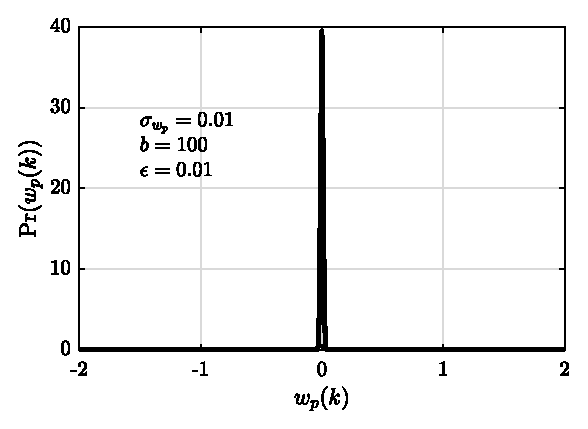
\includegraphics[width=9cm]{alpha-pdf-4.eps}
	\caption{Probability density of a random shock signal}
\end{figure}

The choice of $A(z^{-1})$ and $B(z^{-1})$ in (\ref{eq:RODD}) determines the nature of the RODD disturbance. For example, if $B(z^{-1})=1$ and $A(z^{-1})=1-z^{-1}$, $p(k)$ will be a random walk process with infrequent, large step changes, such as example (a) in Figure \ref{fig:RODDstep}.

\begin{figure}[htp] \label{fig:RODD-examples}
	%... figure contents...
\end{figure}

Denoting $\nabla=1-z^{-1}$, the \textit{RODD step-disturbance} process can be defined as

\begin{equation} \label{eq:RODD-step}
	p(k)= \frac{1}{\nabla}w_p(k)
\end{equation}

The following produces a \textit{RODD ramp-disturbance} consisting of a series of ramps with randomly-occurring changes in slope.

\begin{equation} \label{eq:RODD-ramp}
	p(k)= \frac{1}{\nabla^2}w_p(k)
\end{equation}

The following process with $0<a_1<1$ produces a RODD disturbance consisting of randomly-occurring decaying exponential changes.

\begin{equation} \label{eq:RODD-exp}
	p(k)= \frac{1}{(1-a_1z^{-1})\nabla}w_p(k)
\end{equation}

Examples of these RODD disturbances are also shown in Figure \ref{fig:RODDstep}.


\section{State estimation}

<text>


\section{Model identification}

% Note: may remove this if we aren’t using any formal methods.

<text>


\section{Control strategies}

<text>


\section{Grinding simulation model}

<text>


\section{Performance evaluation}
	
<text>

